\chapter{Background}
\label{chp:background} 

This thesis describes the setup and usage of an End-to-End \gls{iot} system. In order for this to be set up by others later to perform reproducible tests, a detailed description of components, sensors and protocols used is needed. This chapter will go through the background information of the devices and technologies used, and why these where chosen over other alternatives. 

%\section{Internet of Things} % Tjae

%Comment: Read Future Internet: The Internet of Things from 2010.  \cite{gubbi2013internet}

%Comment: Read http://ac.els-cdn.com/S1570870512000674/1-s2.0-S1570870512000674-main.pdf?_tid=6f15526e-eae8-11e5-addc-00000aab0f6b&acdnat=1458072152_0740a71f559cd8ae1ebd0ce4a687e122

%M2M and "M2T" ("Machine to Thing-communication"). Classification of a thing? \cite{tan2010future}. 

%\section{Challenges}

\section{Bluetooth Low Energy}

\gls{ble} is a wireless technology for short range communication developed by the Bluetooth Special Interest Group \cite{gomez2012overview}. The idea was to create a low energy single-hop network solution for \glspl{pan}. A major advantage of this is that Bluetooth 4.0 is already a well established technology in cell phones, laptops and several other devices, and \gls{ble} can use several similarities with this. The 6LoWPAN Working Group has recognized the importance if \gls{ble} in \gls{iot} \cite{hui2008extending}.

The protocol stack of \gls{ble} has two main parts, the controller and the host. In the system used in this thesis this represents the Raspberry Pi as the controller (master) and Nordic nRF52 as the host (slave). The communication between these is done through the standard \gls{hci}. All slaves are in sleep mode by default, and are woken up by the master when communication is needed. Links are being identified by a randomly generated 32-bit code. 

In the case of the network used in this thesis, when the \gls{ble} slave has been connected to a master, it stops searching for other masters, and it is not possible to connect to several masters. This means that we are only able to create a \textit{star network}, not a \textit{mesh network}. This could possibly be an idea for improvement later. Other than this, \gls{ble} seems like a very good alternative in this project. 


\section{6LoWPAN}

%To identify sensors and devices in low energy sensor and device networks, a new protocol was needed. 

\gls{6lowpan} is a defined protocol for using \gls{ipv6} in low enerdy networks, to identify sensors and devices, as defined in the IEEE 802.15.4. 

To use the Internet Protocol was proposed by Geoff Mulligan and the 6LoWPAN Working Group in \cite{mulligan20076lowpan}. In this paper the advantage of \gls{6lowpan} is explained as the easiest way to use standard protocols such as \gls{udp}, \gls{tcp}, \gls{icmp}, gls{dns} and \gls{tftp}, since they can be used directly without the requirement of a translation mechanism. They are already adapted to run over \gls{ipv6}. 

In addition to this, the paper argues that \gls{6lowpan} was developed to be used in small sensor networks. Implementations can fit into 32Kb flash memory parts, wich is smaller than Zigbee and Zensys (which is the two main comparisons made in the paper). It also uses an impressive header comparison mechanism that allows the transmission of \gls{ipv6} packets in 4 bytes, much less than the standard 40 bytes. This is done by using stacked headers, same as in the \gls{ipv6} model, rather than defining a specific header as for \gls{ipv4}. This means that a device can send only the required part of the stack header, and does not need to include header fields for networking and fragmentation \cite{hui2008extending}. 

\gls{6lowpan} was therefore a natural tool to use in this project, in the \gls{ipv6} and \gls{ble} based network. 

%The \gls{6lowpan} architecture was developed to allow \gls{ipv6} packets to be sent over low energy networks.  

\section{Raspberry Pi}

Developed by Element 14, the Raspberry Pi has become a central tool for many people wanting to get started using microcomputers. This was therefore a natural starting point for us as well. 

The Raspberry Pi 2 model B+ is the second generation of its kind, and its \textit{ARMv7 processor} has approximately six times the performance of the predecessor \cite{raspberryPi2}. With a USB Bluetooth dongle connected, it is quite simple to enable both \gls{6lowpan} and \gls{ble}, given that the right Unix kernel has been used in the \gls{os} of the Pi.

Later in this thesis, the processing power of the Pi compared to performing calculations in the end-points will be a central topic for discussion. 

\subsection{Ubuntu Mate}

Along with the Raspberry Pi, we needed a good and stable operating system with a kernel that supported the \gls{6lowpan} architecture. For this, Ubuntu Mate version 15.10 with kernel version 4.15 was chosen, and used on the Raspberry Pi. As other versions of Ubuntu this is Unix based, and has a complete \gls{gui} of a full \gls{os}. 

\section{nRF52}

The nRF52 is developed by Nordic Semiconductor, and is being described as a family of highly flexible, multi-protocol system on chip. 

% Kok 

\cite{nrf52Nordic}

Running at 64MHz it racks up impressive stats: EEMBC Coremark® score of 215 and 58 Coremark®/mA. Built in a cutting edge 55nm process technology the nRF52 Series is architected for todays need for speed, speed to carry out increasingly complex tasks in the shortest possible time and return to sleep, conserving precious battery power. Introducing a Cortex-M4F processor at its heart, it is the most capable Bluetooth Smart SoC on the market today.	
With a brand new multiprotocol radio architecture limits are pushed even further for Bluetooth Smart: A total link budget of 100dBm, -96dBm sensitivity, +4dBm output power and -42dBm selectivity, it is built to exist reliably and effectively in a busy 2.4GHz band. Couple this RF resilience with outstanding power consumption: 5.3mA at 0dBm TX output power and 5.4mA RX it is miserly with power when getting things done on-air.

 

Designed with wealth of digital and analog interfaces and peripherals, there’s something to cover every design requirement. The demands of today’s Bluetooth smart single chip designs are increasingly varied and complex, they can range from digital audio processing, to FFT/FIR and security algorithms, to driving device displays and UIs. Whatever the task, nRF52 series has it covered.

 

We’ve truly made low power easy. We haven’t just just great datasheet numbers, but an automatic and adaptive power management system which combined with extensive EasyDMA and PPI makes the nRF52 Series positively frugal with power.

 

nRF52 Series brings NFC for the first time to a Bluetooth Smart SoC. The on-chip NFC-A tag allows developers to take advantage of NFC ‘touch-to-pair’ functionality in their designs.

 

Maintaining the total flexibility philosophy of the nRF51 Series, it is a flash device. With 512kB flash + 64kB RAM on chip, developers keep all the software stack flexibility and Over-The-Air Device Firmware Upgrade (OTA-DFU) features they enjoyed with the nRF51 Series.

 

We understand that in the world of wearables, size really is everything, so we built a device that is the smallest Bluetooth Smart SoC to date measuring as small as 3.0 x 3.2mm (CSP). With an on-chip balun and a minimum of external components it has the smallest design footprint out there.

 

Tomorrow’s Bluetooth Smart Solutions are going to ask a lot. The nRF52 Series delivers.

% Kok slutt


% https://www.nordicsemi.com/Products/nRF52-Series-SoC

\section{Adafruit ADXL345 Accelerometer}

In order to do collect data, a sensor needed to be connected to the Nordic Semiconductor nRF52. The main thought behind the thesis was to measure vibrations, and a good accelerometer was needed. The Adafruit ADXL345 accelerometer was chosen for several reasons. 

\begin{itemize}
  \item It is the same accelerometer built in on the Zolertia Z1 microcontroller
  \item It can measure acceleration in the axis
  \item It sends digital data directly
  \item It supports both \gls{i2c} and \gls{spi}, which makes it easy to connect to the nRF52. 
\end{itemize}


\begin{figure}[h]
    \centering
    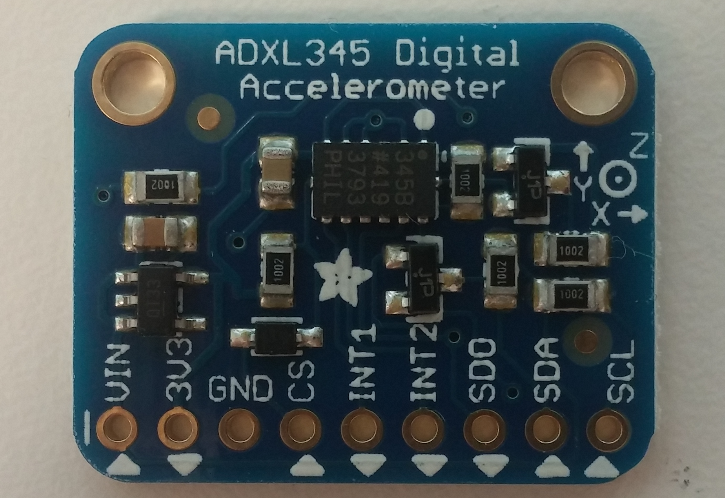
\includegraphics[scale=0.32]{ADXL345.png}    \caption{ADXL345 Accelerometer}
    \label{fig:adxl345}
\end{figure}

\newpage

\section{Transport protocols}



\subsection{\gls{coap}}

The \gls{coap} protocol is described in the documentation as follows: 

\textit{"..a specialized web
   transfer protocol for use with constrained nodes and constrained
   (e.g., low-power, lossy) networks.  The nodes often have 8-bit
   microcontrollers with small amounts of ROM and RAM, while constrained
   networks such as IPv6 over Low-Power Wireless Personal Area Networks
   (6LoWPANs) often have high packet error rates and a typical
   throughput of 10s of kbit/s.  The protocol is designed for machine-
   to-machine (M2M) applications such as smart energy and building
   automation." } \cite{shelby2014constrained}
   


\subsection{\gls{mqtt}}

\section{Software tools}

As \gls{ide}, the \textit{KEIL Vision} was used, as recommended by Nordic Semiconductor (where?), for writing C programming. For other programming languages (for instance Python 3.1) \textit{Sublime Text 2} for Windows and Linux was used, as well as \textit{Pluma} for Ubuntu Mate on the Raspberry Pi. 

%\subsection{Connecting nRF52 and ADXL345}

% Remove to architecture? 




